
\documentclass[12pt, addpoints]{exam}
\usepackage[utf8]{inputenc}
\usepackage[portuguese]{babel}
\usepackage{multicol}
\usepackage{graphicx}
\usepackage{amsmath}

\setlength{\columnsep}{1cm}

\begin{document}

        
\begin{minipage}[l]{0.5\linewidth}
    \begin{flushleft}
        {\bf \Large Prova bimestral}
    \end{flushleft}
\end{minipage}
\begin{minipage}[r]{0.5\linewidth}
    \begin{flushright}
        {\bf \Large Código: XXXXX}
    \end{flushright}
\end{minipage}
\vspace{1cm} \hrule \vspace{0.5cm}
\begin{minipage}{0.70\linewidth}
    Aluno:
\end{minipage}
\begin{minipage}{0.25\linewidth}
    Turma:
\end{minipage}
\vspace{0.5cm} \hrule \vspace{0.5cm}

\begin{questions}
\begin{multicols*}{2}
\question[33] Durante sua trajetória uma partícula realizou um trabalho de    1.95 J. Qual foi a variação da sua energia cinética?

\begin{oneparchoices}
\choice 8.74 J\choice -9.82 J\choice 1.95 J\choice 7.66 J\choice -9.91 J\choice 2.89 J\choice 0.99 J\choice 5.87 J\choice 7.1 J\choice 1.97 J\end{oneparchoices}
\question[23] Considere uma partícula de massa    3.95 kg e velocidade    4.44 m/s. Determine a sua energia cinética.

\begin{center}
\begin{minipage}[c]{0.75\linewidth}
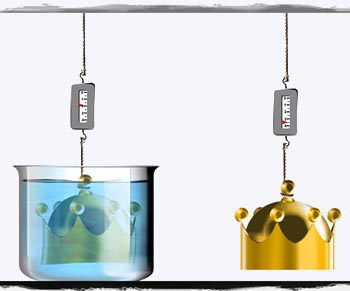
\includegraphics[width=\textwidth]{MWE001.jpg}
\end{minipage}

\end{center}
\begin{oneparchoices}
\choice 108.36 J\choice 15.58 J\choice 22.96 J\choice 100.43 J\choice 3.75 J\choice 38.8 J\choice 495.93 J\choice 18.39 J\choice 5.37 J\choice 170.98 J\end{oneparchoices}
\end{multicols*}
\end{questions}
\newpage
\begin{minipage}[l]{0.5\linewidth}
    \begin{flushleft}
        {\bf \Large Prova bimestral}
    \end{flushleft}
\end{minipage}
\begin{minipage}[r]{0.5\linewidth}
    \begin{flushright}
        {\bf \Large Código: XXXXX}
    \end{flushright}
\end{minipage}
\vspace{1cm} \hrule \vspace{0.5cm}
\begin{minipage}{0.70\linewidth}
    Aluno:
\end{minipage}
\begin{minipage}{0.25\linewidth}
    Turma:
\end{minipage}
\vspace{0.5cm} \hrule \vspace{0.5cm}

\begin{questions}
\begin{multicols*}{2}
\question[33] Durante sua trajetória uma partícula realizou um trabalho de    1.60 J. Qual foi a variação da sua energia cinética?

\begin{oneparchoices}
\choice -3.94 J\choice -7.17 J\choice -1.4 J\choice 0.44 J\choice 4.6 J\choice -1.83 J\choice 7.67 J\choice 1.6 J\choice 1.99 J\choice -6.76 J\end{oneparchoices}
\question[23] Considere uma partícula de massa    4.22 kg e velocidade    2.70 m/s. Determine a sua energia cinética.

\begin{center}
\begin{minipage}[c]{0.75\linewidth}
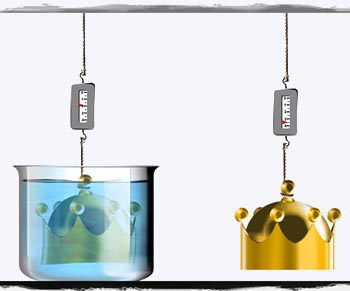
\includegraphics[width=\textwidth]{MWE001.jpg}
\end{minipage}

\end{center}
\begin{oneparchoices}
\choice 104.72 J\choice 54.48 J\choice 396.79 J\choice 6.25 J\choice 15.4 J\choice 127.15 J\choice 378.18 J\choice 266.17 J\choice 18.92 J\choice 137.79 J\end{oneparchoices}
\end{multicols*}
\end{questions}
\newpage
\end{document}
        